\documentclass[10pt]{beamer}
%%
\usepackage{pgfpages}
\usepackage{graphicx}
\usepackage{ulem}
\usepackage{color}
\usepackage{fancyvrb}
\usepackage{listings}
\usepackage{hyperref}
\hypersetup{colorlinks=true}

\lstset{
  language=R,
  % basicstyle=\scriptsize\ttfamily,
  basicstyle=\scriptsize\ttfamily,
  % commentstyle=\ttfamily\color{gray},
  % numbers=none,
%  backgroundcolor=\color{white},
  showspaces=false,
  showstringspaces=false,
%  showtabs=false,
%  frame=single,
  % tabsize=2,
  % captionpos=b,
  breaklines=true
  % breakatwhitespace=false,
%  title=\lstname,
  % escapeinside={},
  % keywordstyle={},
  % morekeywords={}
}

% get rid of junk
\usetheme{default}
\beamertemplatenavigationsymbolsempty
\hypersetup{pdfpagemode=UseNone} % don't show bookmarks on initial view
% font
\usefonttheme{professionalfonts}
\usefonttheme{serif}
% page number
\setbeamertemplate{footline}{%
  \raisebox{5pt}{\makebox[\paperwidth]{\hfill\makebox[20pt]{\color{gray}
        \scriptsize\insertframenumber}}}\hspace*{5pt}}
% add a bit of space at the top of the notes page
\addtobeamertemplate{note page}{\setlength{\parskip}{12pt}}

\setbeamertemplate{blocks}[rounded][shadow=true]

\AtBeginSection{
  \begin{frame}
    \begin{center}
      \structure{\Large \insertsection}
    \end{center}
  \end{frame}
}

\newcommand{\df}{{\it data.frame} }
\newcommand{\gr}{{\it GRanges} }
\newcommand{\dfs}{{\it data.frames} }
\newcommand{\mat}{{\it matrix} }

\title{HGSS Workshop : Analysis and Visualization of Large Genomics Data in R}
\author{Jean Monlong}
\institute{Human Genetics department}
\date{March 28, 2017}

\begin{document}


\begin{frame}[fragile]{Before we begin}
  \begin{block}{On a desktop}
    \begin{enumerate}
    \item Login with your McGill credentials.
    \item Open RStudio
    \item Install the packages and download the data.
    \end{enumerate}
  \end{block}
  \begin{block}{On your laptop}
    Install the packages and download the data.
  \end{block}
  \begin{block}{Packages and data}
    \verb!packagesData.R! available at \url{goo.gl/FJtdXu}.
  \end{block}
\end{frame}

%%%%%%%%%%%%%%%%%%%%
%% Title Slide
\begin{frame}
  \centering
  \titlepage
  \begin{minipage}{.4\textwidth}
    
\includegraphics[width=.8\linewidth]{../imgs/hgssLogo-black.png}
  \end{minipage}
  \hspace{.1\textwidth}
  \begin{minipage}{.4\textwidth}
    
\includegraphics[width=\linewidth]{../imgs/McGill-Logo1.png}
  \end{minipage}

\end{frame}

\begin{frame}{Today's topic}
  \begin{block}{}
    \begin{itemize}
    \item Reading large genomics data.
    \item Analyzing large genomics data.
    \item Visualizing large genomics data.
    \end{itemize}
  \end{block}

  \begin{block}{Let's get started !}
    \begin{enumerate}
    \item Open R/Rstudio or whatever you use.
    \item Prepare a folder for the workshop and set it as working directory.
    % \item Download {\sf dataWS2.RData} from \href{https://drive.google.com/open?id=0BwSxlHpMjRKtflJZejdFZDhkRW5BeUc4VFByWmNMMS1xUEF6ZUFCbFpYTkZEREc1VE5BdGM&authuser=0}{\uline{there}} !!
    \end{enumerate}
  \end{block}

  \begin{alertblock}{Disclaimer}
    \begin{itemize}
    \item Some things might be technical. Follow what you can.
    \item Feel free to interrupt or suggest other ways.
    \item No need to type/do everything.
    \item You can follow the \href{https://www.dropbox.com/s/j28rhx2zj7sjvfj/liveScript.txt?dl=0}{live script}.
    \end{itemize}
  \end{alertblock}


\end{frame}

\begin{frame}[fragile, shrink=10]{Today's packages}
  \begin{alertblock}{Installation}
    \begin{itemize}
    \item Using \verb!install.packages! for CRAN packages.
    \item Using \verb!biocLite! for Bioconductor packages.
    \end{itemize}
  \end{alertblock}
  \begin{exampleblock}{Run this}
\begin{lstlisting}
install.packages(c("data.table","dplyr","ggplot2","parallel",
  "BatchJobs", "parallel", "magrittr"))
source("http://bioconductor.org/biocLite.R")
biocLite(c("GenomicRanges","Rsamtools", "VariantAnnotation",
  "rtracklayer", "Gviz"))
\end{lstlisting}
  \end{exampleblock}
  \begin{block}{Shared folder}
    Use the script in the shared Google Drive folder: \url{goo.gl/FJtdXu}.
  \end{block}
\end{frame}

\begin{frame}[fragile, shrink=10]{Today's data}
  \begin{exampleblock}{Get the data}
\begin{lstlisting}
download.file("ftp://ftp.sanger.ac.uk/pub/gencode/Gencode_human/release_19/gencode.v19.annotation.gtf.gz", "gencode.gtf.gz")

download.file("ftp://ftp.1000genomes.ebi.ac.uk/vol1/ftp/release/20130502/ALL.chr22.phase3_shapeit2_mvncall_integrated_v5a.20130502.genotypes.vcf.gz", "tgp22.vcf.gz")
download.file("ftp://ftp.1000genomes.ebi.ac.uk/vol1/ftp/release/20130502/ALL.chr22.phase3_shapeit2_mvncall_integrated_v5a.20130502.genotypes.vcf.gz.tbi", "tgp22.vcf.gz.tbi")
\end{lstlisting}
  \end{exampleblock}
  \begin{block}{Gencode file}
    \begin{itemize}
    \item Human gene reference annotation: genes, exons, transcipts, ...
    \item More than 2 million lines.
    \item See \href{http://www.ensembl.org/info/website/upload/gff.html}{GTF format}.
    \end{itemize}
  \end{block}
  \begin{block}{1000 Genomes Project}
    \begin{itemize}
    \item Variants: SNPs, indels, structural variants.
    \item Chr 22, $\sim$1 million variants and genotypes across 2500 samples.
    \item See \href{http://www.internationalgenome.org/wiki/Analysis/vcf4.0/}{VCF format}
    \end{itemize}
  \end{block}
\end{frame}

%%%%%%%%%%%%%%%%%%
%%%%%%%%%%%%%%%%%%
%%%%%%%%%%%%%%%%%%
\section{Reading large genomics data}

\begin{frame}[fragile]{{\it data.table} package and {\sf fread}}
  \begin{block}{{\sf fread} function}
    \begin{description}
    \item[+] Very fast.
    \item[+] Usually no need for additional parameters.
    \item[-] Has its specific format ({\it data.table})...
    \item[+] ... which can be converted into \df.
    \item[+] Very fast.
    \end{description}
  \end{block}
  \begin{exampleblock}{Example}
    \begin{lstlisting}
library(data.table)
myDT = fread("myFile.tsv")
myDF = as.data.frame(myDT)

myDT = fread("gunzip -c myFile.tsv.gz")
\end{lstlisting}
  \end{exampleblock}
\end{frame}

\begin{frame}[fragile]{Exercise}
  \begin{enumerate}
  \item Read Gencode file (\verb!gencode.gtf.gz!) with \verb!read.table!.
  \item Same with \verb!fread!.
  \item Have a look at the data.
  \item List the different chromosomes.
  \item How many different gene types ?
  \item How many different genes ?
  \item[$\divideontimes$] How many different genes per gene type ?
  \end{enumerate}
\end{frame}

\begin{frame}[fragile]{Chunk-by-chunk approach}
  \begin{block}{}
    When you can analyze the data in slices.
    \bigskip
    \begin{itemize}
    \item[+] Only a slice of the file in memory.
    \item[-] A bit painful/ugly.
    \end{itemize}
  \end{block}
\bigskip

\begin{block}{}
  \begin{lstlisting}
con = file(file.name)
while(length((chunk.df = read.table(con,nrows=1000)))>0){
... Instructions
}
close(con)
\end{lstlisting}
\end{block}
\end{frame}

\begin{frame}[fragile]{Bioconductor packages}
  \begin{block}{}
    \begin{itemize}
    \item GFF format with \verb!import! ({\it rtracklayer} package).
    \item VCF format with \verb!readVcf! ({\it VariantAnnotation} package).
    \end{itemize}
  \end{block}
  \begin{block}{}
    \begin{description}
    \item[+] Parse the format.
    \item[-] Sometimes parse too much $\rightarrow$ complicated object.
    \item[+] Read indexed files.
    \end{description}
  \end{block}

  \begin{alertblock}{Exercise}
    \begin{enumerate}
    \item Read \verb!gencode.gtf.gz! in another object using \verb!import!.
    \item Have a look at the data.
    \end{enumerate}
  \end{alertblock}
\end{frame}

\begin{frame}{Using file indexing}
  \begin{block}{Why indexing ?}
    To \textbf{quickly import a slice} of a file. In genomics, one region.
  \end{block}
  \bigskip
  \begin{block}{Indexing workflow}
    \begin{enumerate}
    \item Order file by position (chr + start).
    \item Compress with bgzip.
    \item Index.
    \end{enumerate}
  \end{block}
  \bigskip
  \begin{block}{How ?}
    With command lines or with R functions.
  \end{block}
\end{frame}

\begin{frame}[fragile]{Indexing files with R}
  \begin{block}{}
    {\it data.table} package is faster to order large files than conventional R.
  \end{block}
  \bigskip
  \begin{block}{}
  \begin{lstlisting}
library(data.table)
dt = fread("file.bed")
setkey(dt, chr, start)
write.table(dt, file="file-ordered.bed")

library(Rsamtools)
bgzip("file-ordered.bed")
indexTabix("file-ordered.bed.bgz")
  \end{lstlisting}
  \end{block}
\end{frame}

\begin{frame}[fragile]{Using indexed files}
  \begin{block}{}
  \begin{lstlisting}
reg = GRanges(...)

library(VariantAnnotation)
vcf <- readVcf("variants.vcf.gz", "hg19", reg)

library(rtracklayer)
gtf = import(TabixFile("annotation.gtf.bgz"), which=reg)
  \end{lstlisting}
  \end{block}
  \bigskip
  \begin{alertblock}{Exercise}
  \begin{enumerate}
  \item Read variants in VCF between coordinates 30 Mb and 31 Mb.
  \item Order, write, compress and index the gencode file.
  \item[$\divideontimes$] Tile the Mb in 10 bins. In each bin count the number of variants in the VCF.
  \end{enumerate}
  \end{alertblock}
\end{frame}

%%%%%%%%%%%%%%%%%%
%%%%%%%%%%%%%%%%%%
%%%%%%%%%%%%%%%%%%
\section{Analyzing large genomics data}

\begin{frame}[fragile]{Avoid loops, use {\sf sapply/lapply} instead}
  \begin{block}{}
    \begin{description}
    \item[+] Avoid manual init/update of objects.
    \item[+] No temporary object polluting the environment.
    \item[+] More optimized.
    \item[+] Easy to parallelize.
    \item[-] More painful to debug.
    \item[-] An error and everything must be computed again.
    \end{description}
  \end{block}
  \begin{block}{}
  \begin{lstlisting}
perm.l = lapply(1:1000, function(ii){
  data.frame(perm=ii, est=..SOMETHING..)
})

perm.df = do.call(rbind, perm.l)
## or
perm.df = as.data.frame(rbindlist(perm.l))
  \end{lstlisting}
  \end{block}
  \begin{alertblock}{Stupid exercise}
    Sample 10 elements of the gencode annotation and count the number of exons, 100 times.
  \end{alertblock}
\end{frame}

\begin{frame}[fragile]{Parallel processing}
  \begin{block}{Easiest solution with {\it parallel} package}
    \begin{itemize}
    \item Using \verb!mclapply! instead of \verb!lapply!.
    \item \verb!mc.cores=! the number of processors to use.
    \end{itemize}
  \end{block}
  \begin{exampleblock}{Example}
\begin{lstlisting}
perm.l = mclapply(1:1000, function(ii){
  data.frame(perm=ii, est=..SOMETHING..)
}, mc.cores=4)
\end{lstlisting}
  \end{exampleblock}
  \begin{alertblock}{Exercise}
    Parallelize the previous exercise.
  \end{alertblock}
\end{frame}

\begin{frame}{Using computing clusters directly with {\it BatchJobs}}
  \begin{block}{What you need}
    \begin{itemize}
    \item A function that can independently the code
      \begin{itemize}
      \item Load packages.
      \item Load necessary data.
      \item Run the code.
      \end{itemize}
    \item A parameter list (used to define the jobs).
    \item Some global objects (same for all jobs). Optional.
    \item Your favorite cluster configured (or your computer).
    \end{itemize}
  \end{block}
  \begin{block}{More info}
    Checkout \href{http://jmonlong.github.io/PopSV//2-ClusterManagement.md/}{PopSV documentation on BatchJobs}. To use Guillimin, Abacus, Briaree or Mammouth \href{mailto:jean.monlong@mail.mcgill.ca}{ask me} for the configuration files.
  \end{block}
\end{frame}

\begin{frame}[fragile]{BatchJobs example}

  \begin{lstlisting}
library(BatchJobs)

reg = makeRegistry("perm")

jobFun <- function(ii, necessaryData){
    library(...)
    ... Instructions using 'ii' and 'necessaryData'
    data.frame(perm=ii, ...)
}

batchMap(reg, jobFun, 1:10, more.args=list(necessaryData=myData))

submitJobs(reg))

showStatus(reg)

perm.l = reduceResultsList(reg)
  \end{lstlisting}

\end{frame}

\begin{frame}[fragile, shrink=19]{\dfs}
  \begin{block}{}
    \begin{itemize}
    \item Mix between \mat and {\it list}
    \item Array form.
    \item Columns can have different data types.
    \end{itemize}
  \end{block}
  \begin{columns}
    \begin{column}{.5\textwidth}
      \begin{block}{\mat}
\begin{Verbatim}[commandchars=\\\{\}]
      samp1 samp2 samp3
gene1  \color{blue}-1.3  -1.8  -4.1\color{black}
gene2  \color{blue}-1.5  -1.2   4.9\color{black}
\end{Verbatim}
      \end{block}
    \end{column}
    \begin{column}{.5\textwidth}
      \begin{block}{\df}
\begin{Verbatim}[commandchars=\\\{\}]
 gene sample expression
\color{red}gene1  samp1       \color{blue}-1.3\color{black}
\color{red}gene2  samp1       \color{blue}-1.5\color{black}
\color{red}gene1  samp2       \color{blue}-1.8\color{black}
\color{red}gene2  samp2       \color{blue}-1.2\color{black}
\color{red}gene1  samp3       \color{blue}-4.1\color{black}
\color{red}gene2  samp3       \color{blue} 4.9\color{black}
\end{Verbatim}
      \end{block}
    \end{column}
  \end{columns}
  \begin{block}{Pros/Cons}
    \begin{columns}
      \begin{column}{.5\textwidth}
        \begin{description}
        \item[+] Dense representation of large data.
        \item[-] Accepts only one data type.
        \item[-] \underline{manual} combination with other information often required.
        \end{description}
      \end{column}
      \begin{column}{.5\textwidth}
        \begin{description}
        \item[+] Flexible.
        \item[+] Accepts several data types.
        \item[+] Can represent all the data needed for an analysis.
        \item[-] Takes more space/memory due to repetitions.
        \end{description}
      \end{column}
    \end{columns}
  \end{block}
\end{frame}

\begin{frame}[fragile]{{\it dplyr} package}
  \begin{block}{``A Grammar of Data Manipulation''}
    {\it dplyr} provides functions which can be combined for data manipulation.
    \begin{description}
    \item[mutate] add a new column using others.
    \item[filter] filter rows (similar as \verb!subset! function).
    \item[select] select specific columns only.
    \item[arrange] order rows using specific columns.
    \item[group\_by] groups rows according to specific columns.
    \item[summarize] summarizes each group of rows.
    \item[do] applies a function to a group of rows.
    \end{description}
  \end{block}
  \begin{block}{}
    \begin{description}
      \item[+] Works with pipes.
      \item[+] Fast.
      \item[-] Has its own format {\it tbl\_df}...
      \item[+] ... which is almost the same as \df.
    \end{description}
  \end{block}
\end{frame}

\begin{frame}[fragile]{Pipes are cool !}
  \begin{block}{}
    \begin{itemize}
    \item Pipe functions instead of embedding them.
    \item More readable.
    \item Easier to combine several functions.
    \item Avoid temporary objects.
    \item Pipe argument \verb!%>%!.
    \end{itemize}
  \end{block}
  \begin{exampleblock}{Example}
\begin{Verbatim}[commandchars=\\\{\}]
head(sort(round(sqrt(myVec))))
myVec \color{blue}%>%\color{black} sqrt \color{blue}%>%\color{black} round \color{blue}%>%\color{black} sort \color{blue}%>%\color{black} head

head(\color{blue}sort(\color{red}round(\color{black}sqrt(myVec)\color{red},digits=3)\color{blue},decreasing=TRUE)\color{black},10)
myVec \color{blue}%>%\color{black} sqrt \color{blue}%>%\color{black} round(digits=3) \color{blue}%>%\color{black}
                        sort(decreasing=TRUE) \color{blue}%>%\color{black} head(10)
\end{Verbatim}
  \end{exampleblock}
\end{frame}

\begin{frame}[fragile]{Grouping rows}
  \begin{block}{Operation by block}
    \begin{itemize}
    \item Using \verb!group_by()! function.
    \item Further operations are applied separately per group of rows.
    \end{itemize}
  \end{block}
  \begin{exampleblock}{Example}
\begin{lstlisting}
myDF %>% group_by(colA) %>% summarize(colB.mean=mean(colB))

myDF %>% group_by(colA, colB) %>% summarize(nbAB=n())

myDF %>% group_by(colAB) %>% summarize(nbAB=n()) %>%
                 ungroup %>% arrange(desc(nbAB)) %>% head
\end{lstlisting}
  \end{exampleblock}
  \begin{block}{Tips}
    \begin{itemize}
    \item \verb!n()! gives the number of rows in the group.
    \item \verb!ungroup! removes groups.
    \item \verb!desc()! means descending order (in \verb!arrange()!).
    \end{itemize}
  \end{block}
\end{frame}

\begin{frame}[fragile]{Exercise}
  \begin{enumerate}
  \item For each gene, compute the number of exon.
  \item Print the top 10 genes with the most exons.
  \item For each gene type, compute the average number of exon per gene.
  \item For each gene type, compute the average gene size.
  \item For each chromosome, compute the number of genes for each gene type.
  \item In protein-coding genes, compute the median size of the first exon, second exon, etc (i.e. per \verb!exon_number!).
  \end{enumerate}
\end{frame}

\begin{frame}[fragile]{GenomicRanges}
  \begin{block}{Introduction}
    Represents genomic intervals. All annotation can be represented through {\it GenomicRanges} objects.
  \end{block}
  \begin{block}{Which function fit your exact need ?}
    \begin{description}
    \item[overlapsAny] Test overlaps of one \gr into second \gr.
    \item[countOverlaps] For each region in one \gr, count how many overlaps from another.
    \item[findOverlaps] Finds overlaps between two {\it GRanges} objects.
    \item[distanceToNearest] Computes the distance from each regions in a {\it GRanges} object to the nearest in another {\it GRanges} object.
    \item[subsetByOverlaps] Keep the regions from one \gr that overlaps another.
    \end{description}
  \end{block}
\end{frame}

\begin{frame}[fragile, shrink=10]{Overlaps between two {\it GRanges} sets}
  \begin{block}{{\sf findOverlaps} function}
    \begin{itemize}
    \item Two {\it GRanges} objects as input.
    \item Extra parameters available for specific overlaps.
    \item Returns the index of regions in object 1 and 2 that overlap.
    \item \verb!queryHits! and \verb!subjectHits! functions to retrieves those index.
    \end{itemize}
  \end{block}
  \begin{exampleblock}{Example}
\begin{lstlisting}
> ol12 = findOverlaps(gr1, gr2)
> ol12
Hits of length 3
queryLength: 6
subjectLength: 4
  queryHits subjectHits
   <integer>   <integer>
 1         1           1
 2         2           2
 3         5           3
> queryHits(ol12)
[1] 1 2 5
\end{lstlisting}
  \end{exampleblock}

\end{frame}

\begin{frame}[fragile]{Better one big overlap than many small ones}
  \begin{alertblock}{Exercise}
    \begin{enumerate}
    \item For each gene type, how many genes have at least one variant in their body ?
    \item[$\divideontimes$] For each gene type, what is the average number of variant per gene ?
    \item[$\divideontimes$] For each gene type, what is the average allele frequency of the variant ?
    \end{enumerate}
  \end{alertblock}

  \begin{block}{Hints}
    \verb!lapply!, \verb!tapply!, {\it dplyr}.
  \end{block}
\end{frame}

\begin{frame}[fragile]{Other tricks}
  \begin{itemize}
  \item Create a {\it GRanges} from a \df.
  \item Change chromosome names ('chr' or no 'chr', that is the question).
  \end{itemize}
  \begin{block}{}
  \begin{lstlisting}
library(GenomicRanges)

gr = makeGRangesFromDataFrame(df, keep.extra.columns = TRUE)

seqlevels(genc) = gsub("chr","",seqlevels(genc))
## or
seqlevels(genc) = paste0("chr",seqlevels(genc))
  \end{lstlisting}
  \end{block}
\end{frame}

\begin{frame}[fragile]{{\it GenomicRanges} + {\it dplyr}}
  \begin{block}{{\sf tapply}}
    \begin{enumerate}
    \item The values to use (vector).
    \item How to group these values (vector).
    \item The function to run (input is one vector).
    \end{enumerate}
  \end{block}
  \begin{block}{}
  \begin{lstlisting}
tapply(...subjectHits(ol)..., ...queryHits(ol)..., function(x)...)

ol %>% as.data.frame %>% mutate(...queryHits..., ...subjectHits...) %>% group_by(...) %>% summarize(...)
  \end{lstlisting}
  \end{block}
  \begin{block}{}
    \verb!tapply! works but {\it dplyr} is faster and more flexible.
  \end{block}
\end{frame}

%%%%%%%%%%%%%%%%%%
%%%%%%%%%%%%%%%%%%
%%%%%%%%%%%%%%%%%%
\section{Visualizing large genomics data}

\begin{frame}[fragile]{{\it Gviz} for multi-track graphs}
  \begin{block}{}
  \begin{lstlisting}
library(Gviz)

gatrack = GenomeAxisTrack()
snp.t = DataTrack(snp.gr, data="AF", type='h', name="SNP freq")
plotTracks(list(gatrack, snp.t))
  \end{lstlisting}

  \end{block}

  \begin{block}{More info}
    See slides/code/links from \href{https://github.com/jmonlong/MonBUG17_Gviz}{MonBUG Gviz demo}.
  \end{block}
\end{frame}

\begin{frame}{{\sf ggplot2} package}
  \begin{block}{Introduction}
    A package to construct pretty and/or complex graphs. Many aspects of the graph are arranged automatically but everything can be specified. Easy layers addition.
  \end{block}

  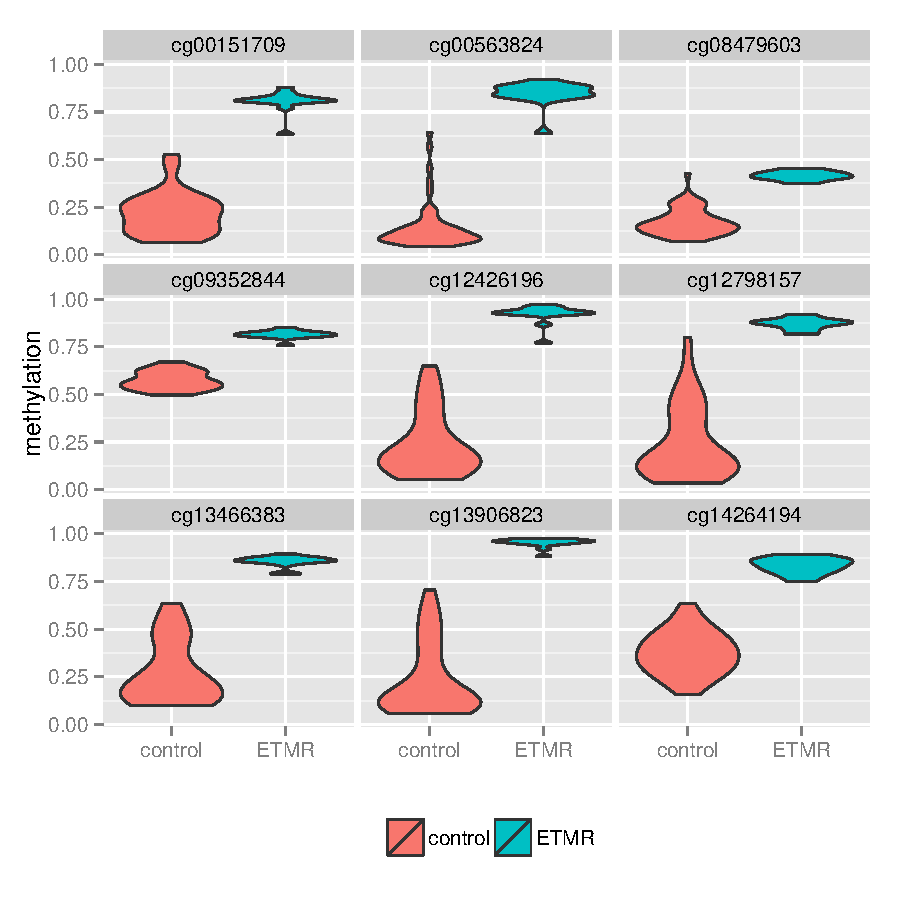
\includegraphics[height=.6\textheight]{../imgs/example-ggplot2.pdf}
  \includegraphics[height=.6\textheight,page=2]{../imgs/example-ggplot2.pdf}

\end{frame}

\begin{frame}[fragile, shrink=10]{{\sf ggplot2}}
  \begin{block}{Input : \df}
    \begin{itemize}
    \item Each row represents one {\it "observation"}.
    \item Columns represent the different information about the {\it "observations"}.
    \end{itemize}
  \end{block}

  \begin{block}{Concept}
    \begin{itemize}
    \item Start with a \verb!ggplot(...)! part and the input \df.
    \item \verb!aes(...)! defines how to use the input \df columns.
    \item Add layers : \verb!geom_*(...)!, \verb!scale_*(...)!, ...
    \end{itemize}
  \end{block}

  \begin{exampleblock}{Example}
\begin{Verbatim}[commandchars=\\\{\}]
library(ggplot2)
\color{blue}ggplot(\color{red}myDf\color{black}\color{blue}, aes(\color{black}x=\color{red}colA\color{black}, y=\color{red}colB\color{black}, colour=\color{red}colC\color{black}, linetype=\color{red}colD\color{black}\color{blue}))
   + geom_point() + geom_line() + scale_y_log10()
\end{Verbatim}
  \end{exampleblock}

  \begin{block}{Useful online resources}
    \begin{itemize}
    \item \url{http://docs.ggplot2.org/current/}
    \item \url{http://www.cookbook-r.com/Graphs/}
    \end{itemize}
  \end{block}

\end{frame}

\begin{frame}{Exercise}
  \begin{enumerate}
  \item Show the distribution of the gene size (histogram), colored by gene type.
  \item Show for each chromosome the number of genes, colored by gene type.
  \item[$\divideontimes$] Show the median size of the first exon, second exon, etc, of protein coding genes.
  \item[$\divideontimes$] For each gene type, what is the average allele frequency of the variant ? Maybe a boxplot ?
  \end{enumerate}
\end{frame}

\begin{frame}{Final recommendations}
  \begin{itemize}
  \item Use \textbf{names} that makes sense (to you and future you).
  \item \textbf{Nothing in the console}, everything in an organized script.
  \item The script should be \textbf{sequential and commented} when complex.
  \item Save the graphs \textbf{in the code}, not manually through RStudio.
  \item \textbf{Split} long scripts and \textbf{save} temporary files.
  \item \textbf{Overwriting} is fine if in the same paragraph.
  \item Use \textbf{functions/pipes} to avoid environment/code pollution.
  \item Use \textbf{R Markdown} to produce a readable report while keeping the code.
  \end{itemize}
\end{frame}

\end{document}


%%% Local Variables:
%%% mode: latex
%%% TeX-master: t
%%% End:
